
\section{Conception du logiciel}

Le logiciel se décompose en trois blocs principaux~:
\begin{itemize}
    \item L'objet paramètrique
    \item Les lumières
    \item La gestion des entrées/sorties (fenêtre)
\end{itemize}

On notera également l'existence des classes \textit{VBO} et \textit{shader\_program}, qui sont de
simples wrappers autours d'OpenGL pour faciliter son utilisation (en gérant par exemple
les vérifications d'erreur et la libération des ressources)

[voir UML page suivante]

\begin{landscape}
    \thispagestyle{empty}
    \begin{figure}[h]
        \centering
        \fbox{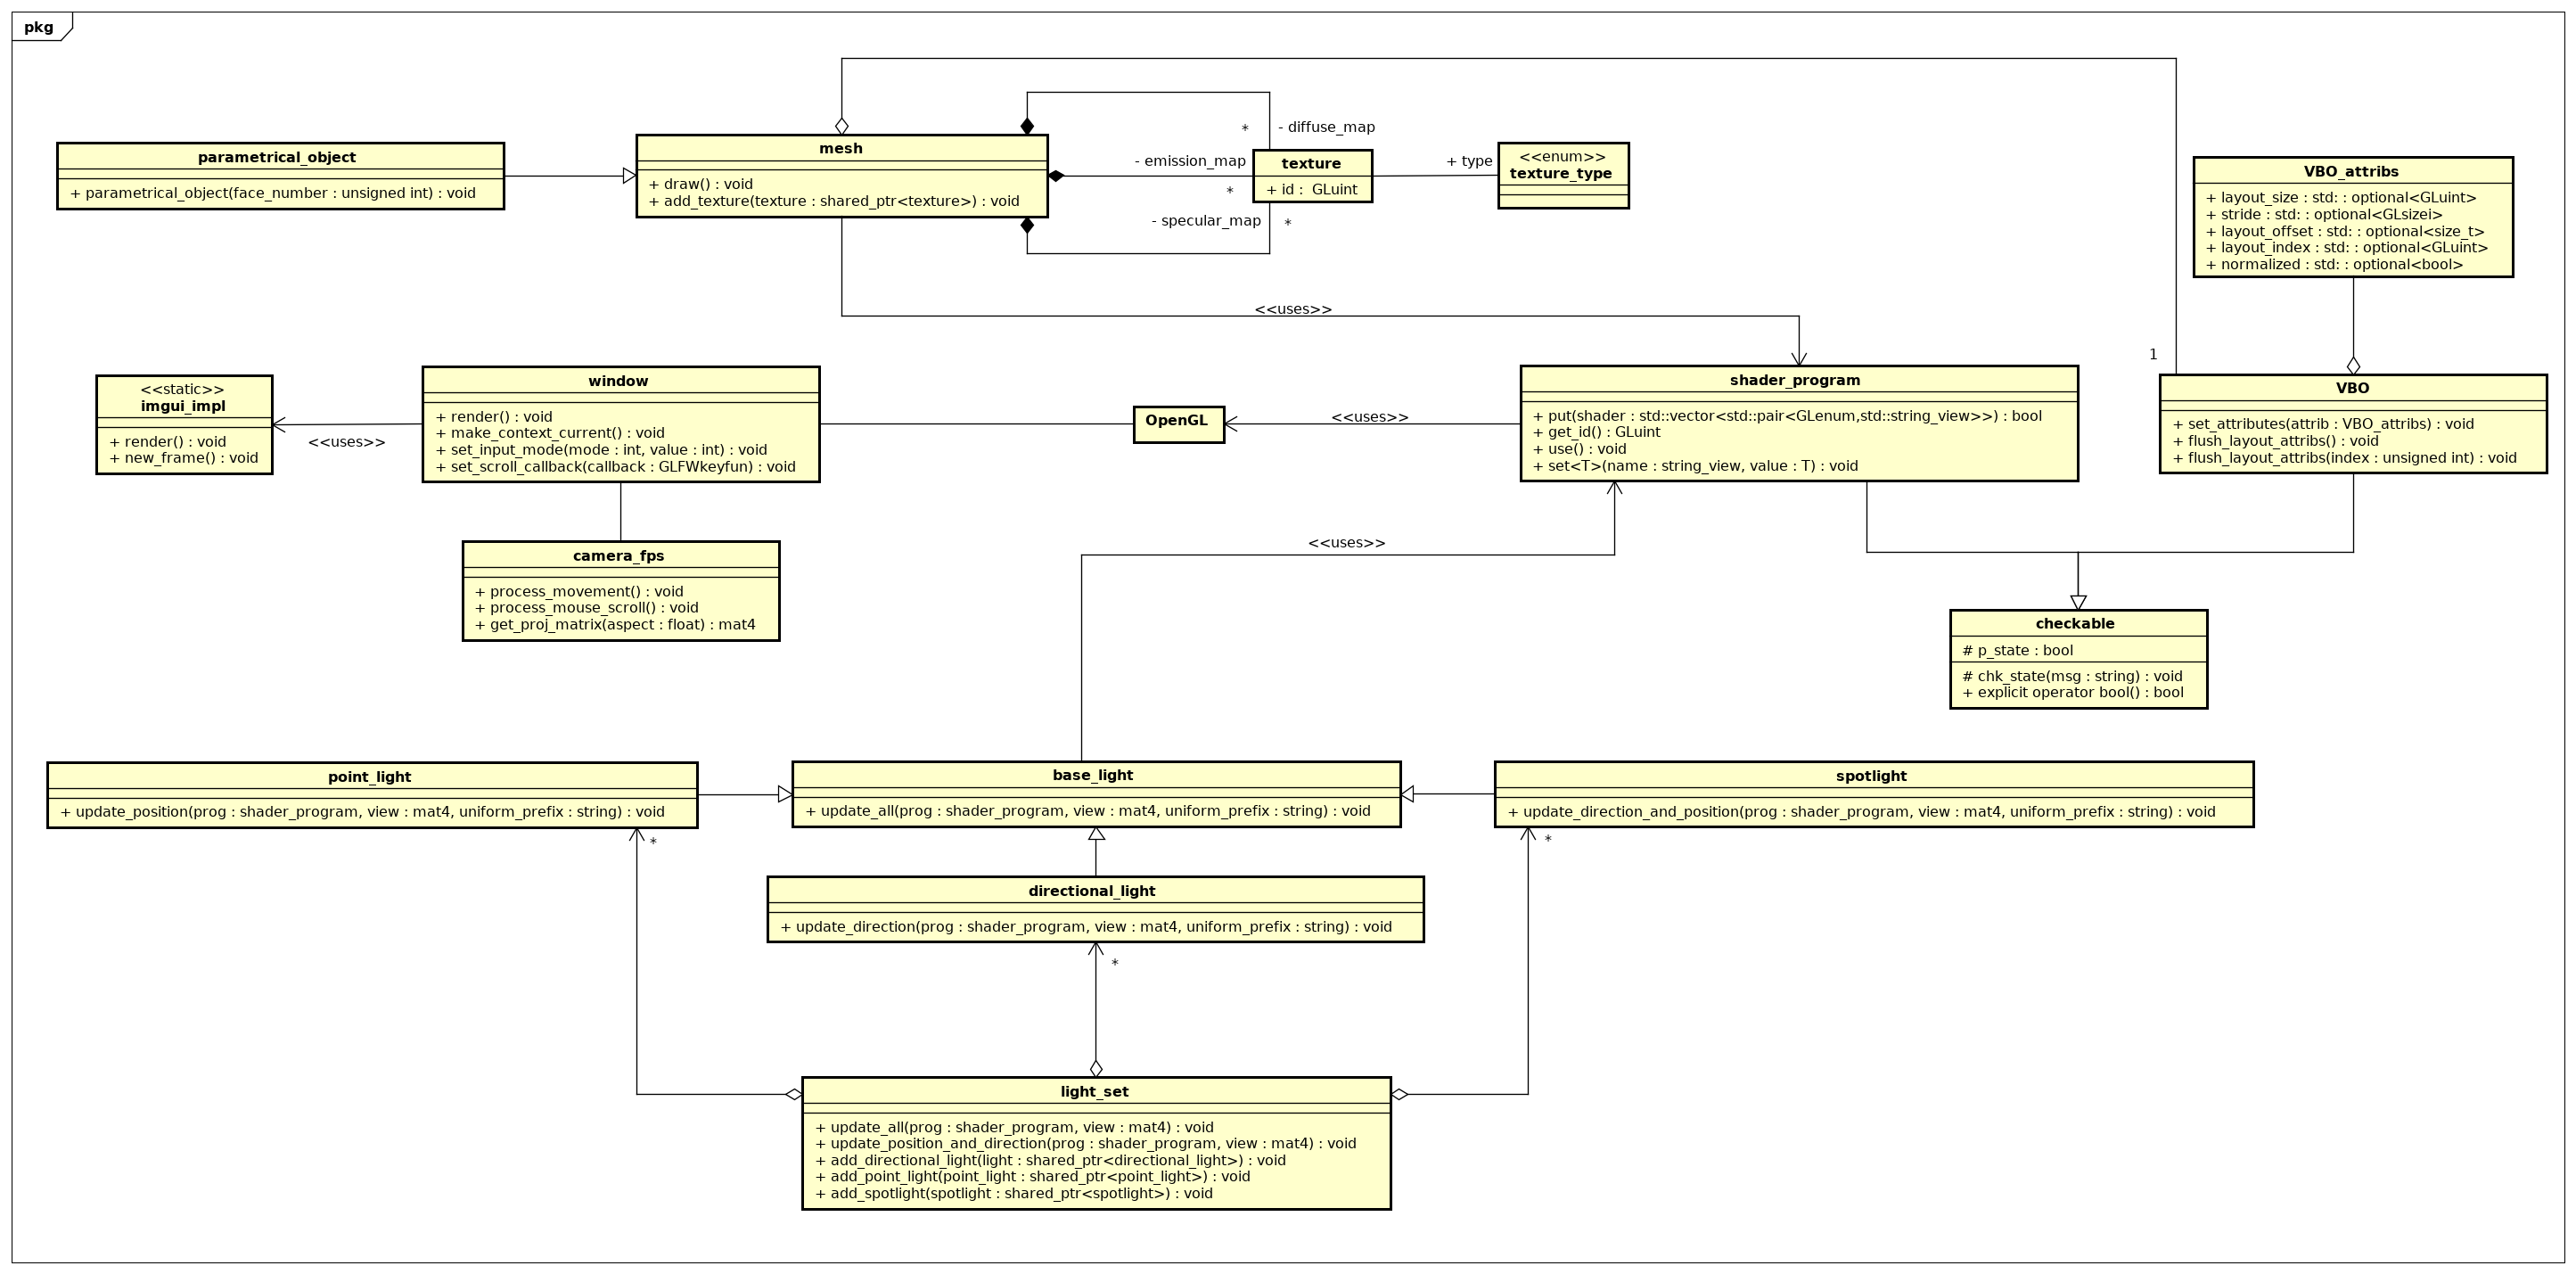
\includegraphics[width=1\linewidth, height=1\textheight,keepaspectratio]{UML.png}}
    \end{figure}
\end{landscape}

\subsection{Objet Paramétrique}

L'objet paramétrique est construit à partir d'un entier \(n\) représentant le
nombre de faces sur la partie inférieure d'un diamant. À l'instanciation, il génère un
tableau de vertices et un d'indices représentant le-dit diamant.

\subsection{Lumières}

Les lumières sont découpées en types~:
\begin{itemize}
    \item \textit{point\_light} qui diffuse une lumière autours d'un point
    \item \textit{directional\_light} qui génère une lumière directionelle
        unie (façon soleil)
    \item \textit{spotlight} qui émet une lumière en cône à partir d'un point
\end{itemize}
La classe \textit{light\_set} est une simple classe utilitaire utilisée pour
gérer tous les éclairages à la fois

\subsection{Fenêtre}
La classe \textit{window} est une classe qui nous permet d'initialiser les
différentes bibliothèques gérant l'affichage~:
\begin{itemize}
    \item \textit{imgui}, qui gère les bouttons, les barres de défilement, …
    \item \textit{glad}, qui s'occupe de charger OpenGL
    \item \textit{glfw}, qui permet d'ouvrir la fenêtre et de récupérer les
        entrées clavier/souris
\end{itemize}


